%%%%%%%%%%%%%%%%%%%%%%%%%%%%%%%%%%%%%%%%%
% Short Sectioned Assignment LaTeX Template Version 1.0 (5/5/12)
% This template has been downloaded from: http://www.LaTeXTemplates.com
% Original author:  Frits Wenneker (http://www.howtotex.com)
% License: CC BY-NC-SA 3.0 (http://creativecommons.org/licenses/by-nc-sa/3.0/)
%%%%%%%%%%%%%%%%%%%%%%%%%%%%%%%%%%%%%%%%%

%----------------------------------------------------------------------------------------
%	PACKAGES AND OTHER DOCUMENT CONFIGURATIONS
%----------------------------------------------------------------------------------------

\documentclass[paper=a4, fontsize=11pt]{scrartcl} % A4 paper and 11pt font size

% ---- Entrada y salida de texto -----

\usepackage[T1]{fontenc} % Use 8-bit encoding that has 256 glyphs
\usepackage[utf8]{inputenc}
%\usepackage{fourier} % Use the Adobe Utopia font for the document - comment this line to return to the LaTeX default

% ---- Idioma --------

\usepackage[spanish, es-tabla]{babel} % Selecciona el español para palabras introducidas automáticamente, p.ej. "septiembre" en la fecha y especifica que se use la palabra Tabla en vez de Cuadro

% NOTA: en caso de problema al compilar, compruebe que tiene el paquete: texlive-babel-spanish.noarch

% ---- Otros paquetes ----

\usepackage{amsmath,amsfonts,amsthm} % Math packages
\usepackage{graphics,graphicx,floatrow} %para incluir imágenes y notas en las imágenes
\usepackage{listings}

\usepackage{url}

%% Define a new 'leo' style for the package that will use a smaller font.
\makeatletter
\def\url@leostyle{%
	\@ifundefined{selectfont}{\def\UrlFont{\sf}}{\def\UrlFont{\small\ttfamily}}}
\makeatother
%% Now actually use the newly defined style.
\urlstyle{leo}
\setlength{\parindent}{12pt}

% Para hacer tablas comlejas
\usepackage{multirow}
\usepackage{threeparttable}

%\usepackage{sectsty} % Allows customizing section commands
%\allsectionsfont{\centering \normalfont\scshape} % Make all sections centered, the default font and small caps

\usepackage{fancyhdr} % Custom headers and footers
\pagestyle{fancyplain} % Makes all pages in the document conform to the custom headers and footers
\fancyhead{} % No page header - if you want one, create it in the same way as the footers below
\fancyfoot[L]{} % Empty left footer
\fancyfoot[C]{} % Empty center footer
\fancyfoot[R]{\thepage} % Page numbering for right footer
\renewcommand{\headrulewidth}{0pt} % Remove header underlines
\renewcommand{\footrulewidth}{0pt} % Remove footer underlines
\setlength{\headheight}{13.6pt} % Customize the height of the header

\numberwithin{equation}{section} % Number equations within sections (i.e. 1.1, 1.2, 2.1, 2.2 instead of 1, 2, 3, 4)
\numberwithin{figure}{section} % Number figures within sections (i.e. 1.1, 1.2, 2.1, 2.2 instead of 1, 2, 3, 4)
\numberwithin{table}{section} % Number tables within sections (i.e. 1.1, 1.2, 2.1, 2.2 instead of 1, 2, 3, 4)

\setlength\parindent{0pt} % Removes all indentation from paragraphs - comment this line for an assignment with lots of text

\newcommand{\horrule}[1]{\rule{\linewidth}{#1}} % Create horizontal rule command with 1 argument of height



\usepackage[utf8]{inputenc}
\usepackage[T1]{fontenc}
\usepackage[spanish]{babel}
\usepackage{times}

\usepackage{color}
\definecolor{gray97}{gray}{.97}
\definecolor{gray75}{gray}{.75}
\definecolor{gray45}{gray}{.45}

\usepackage{listings}
\lstset{ frame=Ltb,
	framerule=0pt,
	aboveskip=0.5cm,
	framextopmargin=3pt,
	framexbottommargin=3pt,
	framexleftmargin=0.4cm,
	framesep=0pt,
	rulesep=.4pt,
	backgroundcolor=\color{gray97},
	rulesepcolor=\color{black},
	%
	stringstyle=\ttfamily,
	showstringspaces = false,
	basicstyle=\small\ttfamily,
	commentstyle=\color{gray45},
	keywordstyle=\bfseries,
	%
	numbers=left,
	numbersep=15pt,
	numberstyle=\tiny,
	numberfirstline = false,
	breaklines=true,
}

% minimizar fragmentado de listados
\lstnewenvironment{listing}[1][]
{\lstset{#1}\pagebreak[0]}{\pagebreak[0]}

\lstdefinestyle{consola}
{basicstyle=\scriptsize\bf\ttfamily,
	backgroundcolor=\color{gray75},
}

\lstdefinestyle{C}
{language=C,
}


\usepackage[pdftex,colorlinks=true,linkcolor=negro,urlcolor=blue]{hyperref,xcolor}
\definecolor{negro}{rgb}{0,0,0}

\graphicspath{ {./imagenes/} }
\usepackage{subfig}
\hypersetup{citecolor=blue}

\title{	
\normalfont \normalsize 
\textsc{{\bf Ingeniería de Servidores (2014-2015)} \\ Grado en Ingeniería Informática \\ Universidad de Granada} \\ [25pt]
\horrule{0.5pt} \\[0.4cm] % Thin top horizontal rule
\huge Memoria Práctica 3 \\ % The assignment title
\horrule{2pt} \\[0.5cm] % Thick bottom horizontal rule
}

\author{Jose Antonio Jiménez Montañés}

\date{\normalsize\today}

%----------------------------------------------------------------------------------------
% DOCUMENTO
%----------------------------------------------------------------------------------------
%
%\begin{figure}[H]
%	\centering
%	\includegraphics[width=0.5\textwidth]{gull}
%	\caption{Texto Prueba}
%	\label{fig:ddd}
%\end{figure}


%\cite{p1}


\begin{document}

\maketitle % Muestra el Título

\newpage %inserta un salto de página

\tableofcontents % para generar el índice de contenidos
\clearpage
\listoffigures

%\listoftables 

\newpage

%----------------------------------------------------------------------------------------
%	Cuestion 1
%----------------------------------------------------------------------------------------

\section {a) ¿Qué archivo le permite ver qué programas se han instalado con el gestor de paquetes? b) ¿Qué significan las terminaciones. 1.gz o .2.gz de los archivos en ese directorio?}


a) En Ubuntu Server esta localizado en: /var/logs/apt/history.log

\begin{figure}[H]
	\centering
	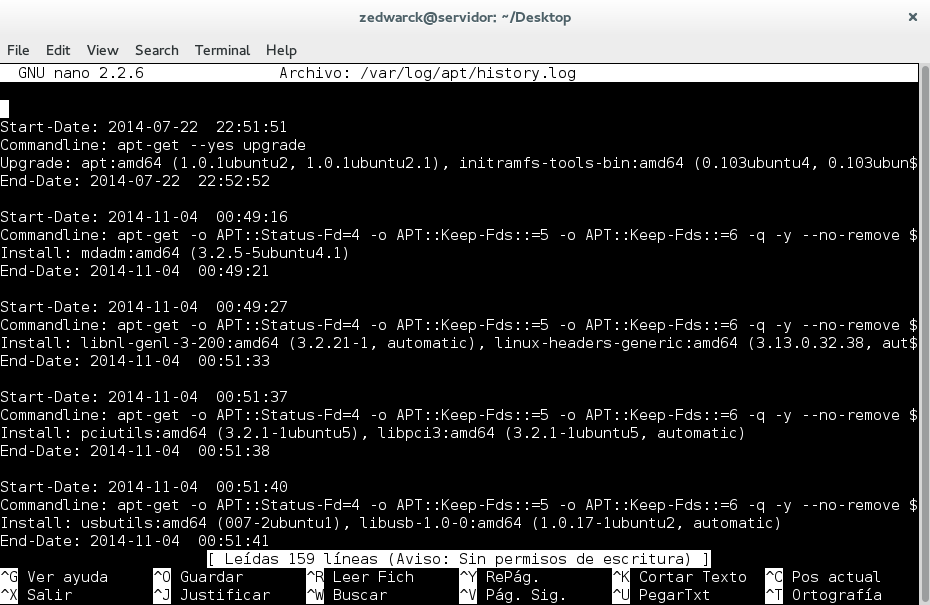
\includegraphics[width=1\textwidth]{c01f01}
	\caption{Contenido de history.log}
	\label{fig:c01f01}
\end{figure}


b) El nivel de compresión gzip utilizado.


%------------------------------------------------
% CUESTION OPCIONAL 1
%------------------------------------------------
\section{Indique qué comandos ha utilizado para realizarlo así como capturas de pantalla del proceso de reconstrucción del RAID. \cite{c01o}}

Comprobamos primero que funciona el RAID1 y eliminamos el disco2. Comprobamos que detecta que el disco 2 falla: (Lo hemos eliminado)

\begin{figure}[H]
	\centering
	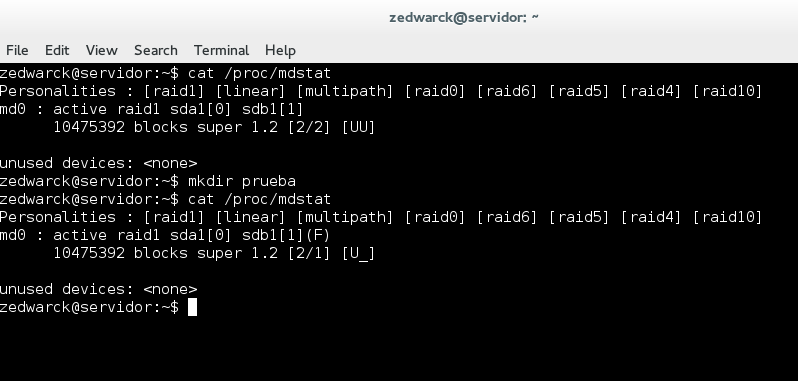
\includegraphics[width=1\textwidth]{co01f01}
	\caption{Sistema detecta que el RAID falla}
	\label{fig:co01f01}
\end{figure}


Si el disco diera fallos lógicos debería ser retirado con: "sudo mdadm --remove /dev/md0 /dev/sdb1"\\

De una forma u de otra el siguiente paso sería retirarlo del sistema con: "sudo mdadm --manage /dev/md0 --remove /dev/sdb1"\\

Luego procedemos a instalar el nuevo disco que ya debería estar en el sistema con: "sudo mdadm --add /dev/md0 /dev/sdb1"\\

Comprobamos que ahora esta el disco en el sistema RAID y esta actualizando datos:

\begin{figure}[H]
	\centering
	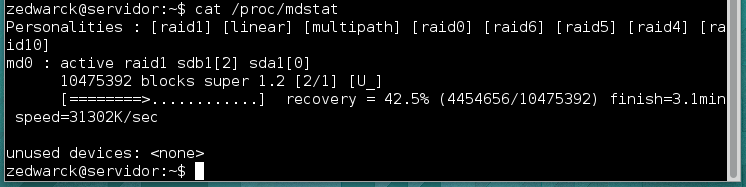
\includegraphics[width=1\textwidth]{co01f02}
	\caption{Sistema detecta nuevo disco en RAID y lo actualiza}
	\label{fig:co01f02}
\end{figure}


%----------------------------------------------------------------------
% CUESTION 2	
%----------------------------------------------------------------------------------------

\section{¿Qué archivo ha de modificar para programar una tarea? Escriba la línea necesaria para ejecutar una vez al día una copia del directorio \~/codigo a \~/seguridad/\$fecha donde \$fecha es la fecha actual	(puede usar el comando date). \cite{c02}}

Se crea o se modifica el archivo de tareas con "crontab -e", aunque si ya lo hemos creado alguna vez estará situado en: /var/spool/cron/usuario\\

Una vez creado, el demonio cron se ejecuta cada cierto tiempo(a las 5am en nuestro caso) y ejecuta la tarea que le hemos indicado, en nuestro caso: creación de un directorio con la fecha actual y copia del contenido de "codigo" dentro del directorio creado en "seguridad"

\begin{figure}[H]
	\centering
	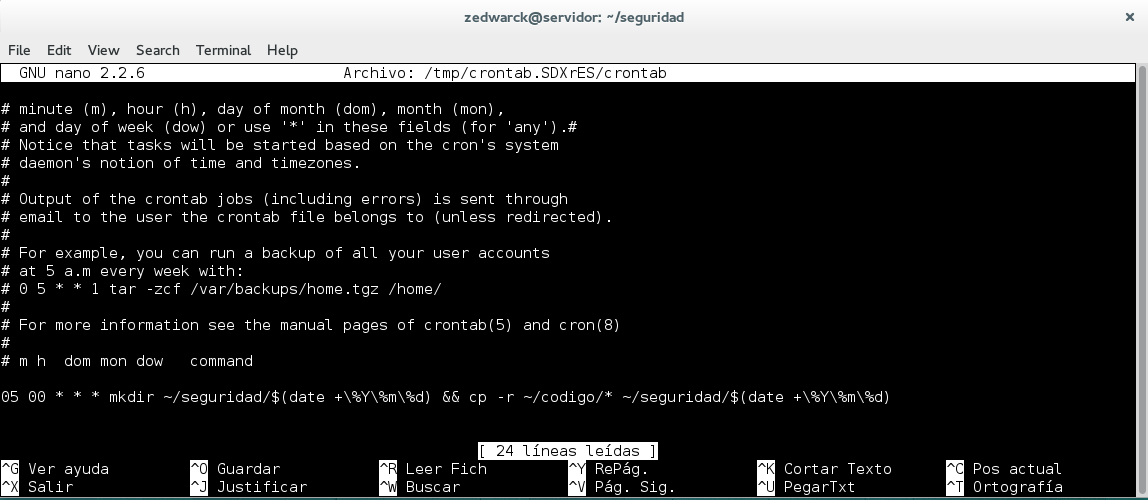
\includegraphics[width=1\textwidth]{c02f01}
	\caption{Configuracion del crontab para la tarea diaria.}
	\label{fig:c02f01}
\end{figure}



%-------------------------------------------------------------------------------------------
% CUESTION 3
%--------------------------------------------------------------------------------------------
\section{Pruebe a ejecutar el comando, conectar un dispositivo USB y vuelva a ejecutar el comando. Copie y pegue la salida del comando. (considere usar dmesg | tail). Comente qué observa en la información mostrada.}

Usamos el comando: "dmesg | tail -10" para visualizar las 10 ultimas lineas del archivo de logs:

\begin{figure}[H]
	\centering
	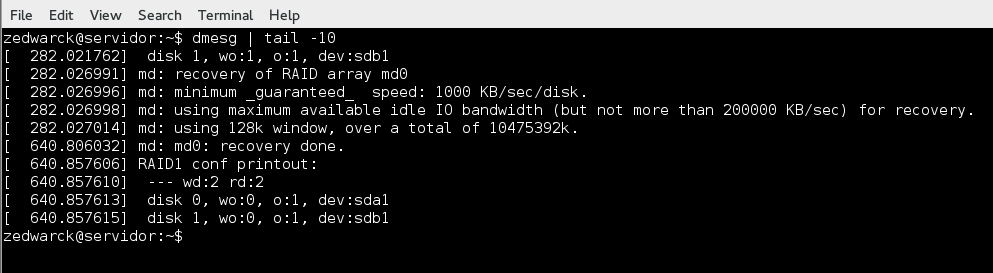
\includegraphics[width=1\textwidth]{c03f01}
	\caption{Últimos registros Hardware del sistema(Antes de introducir USB).}
	\label{fig:c03f01}
\end{figure}

Luego insertamos un dispositivo USB y volvemos a visualizar el archivo:

\begin{figure}[H]
	\centering
	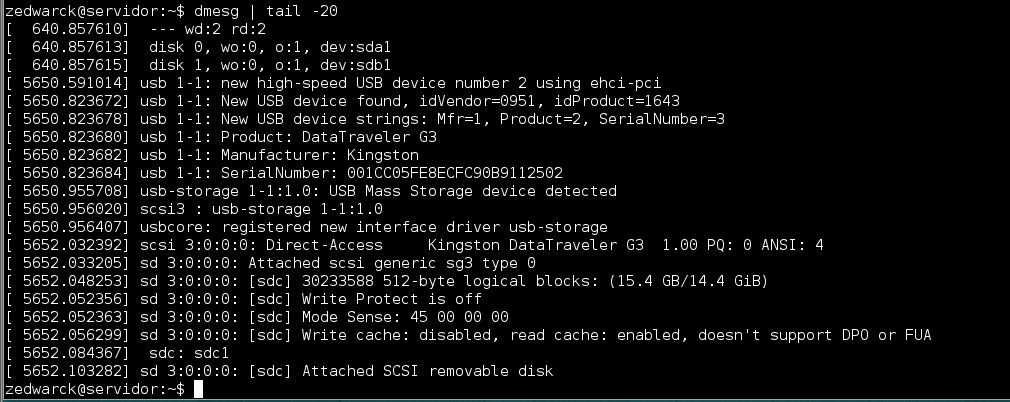
\includegraphics[width=1\textwidth]{c03f02}
	\caption{Últimos registros Hardware del sistema(Después de introducir USB).}
	\label{fig:c03f02}
\end{figure}

Podemos observar como nos da información detallada acerca del dispositivo incluyendo su numero de serie, capacidad, marca, modelo, cache, etc.

%----------------------------------------------------------------------------------------
% CUESTION 4
%----------------------------------------------------------------------------------------
\section{Ejecute el monitor de “System Performance” y muestre el resultado. Incluya capturas de pantalla comentando la información que aparece.}


\begin{figure}[H]
	\centering
	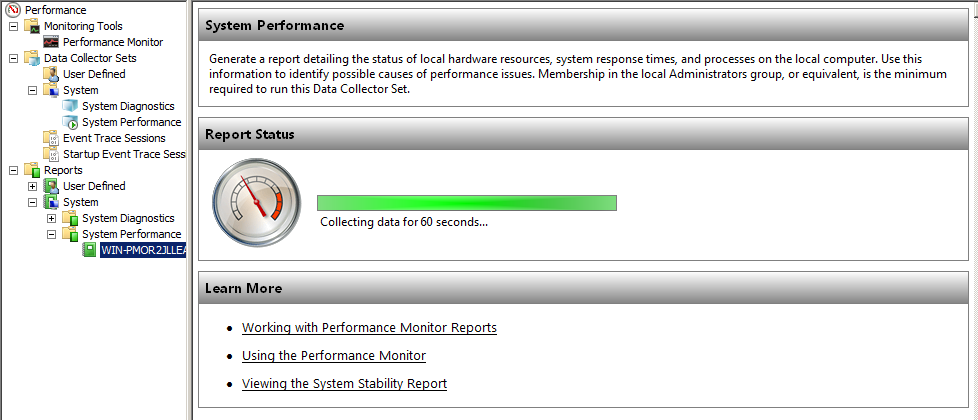
\includegraphics[width=1\textwidth]{c04f01}
	\caption{Esperando a que capture los datos para obtener los resultados.}
	\label{fig:c04f01}
\end{figure}
\begin{figure}[H]
	\centering
	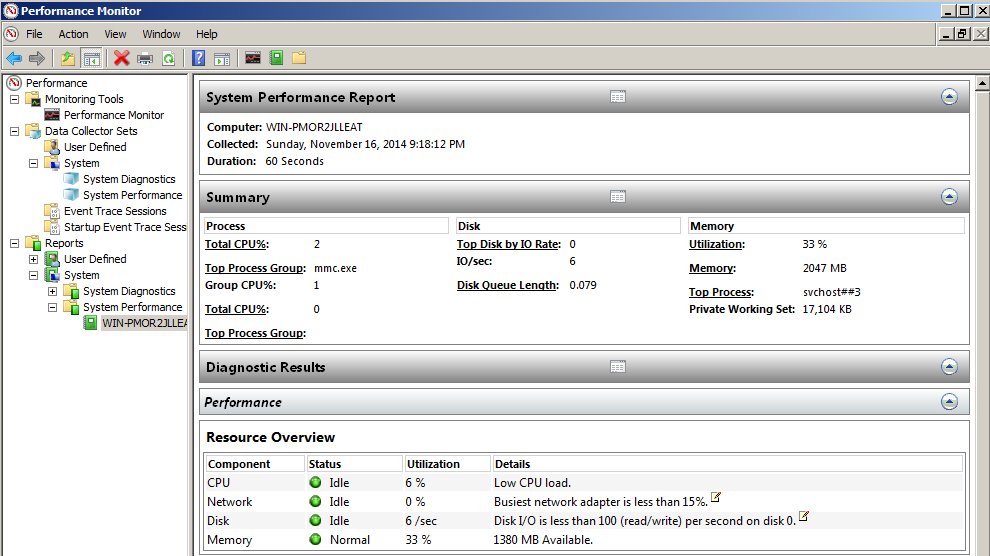
\includegraphics[width=1\textwidth]{c04f02}
	\caption{Resumen del contenido de datos regidos.}
	\label{fig:c04f02}
\end{figure}
\begin{figure}[H]
	\centering
	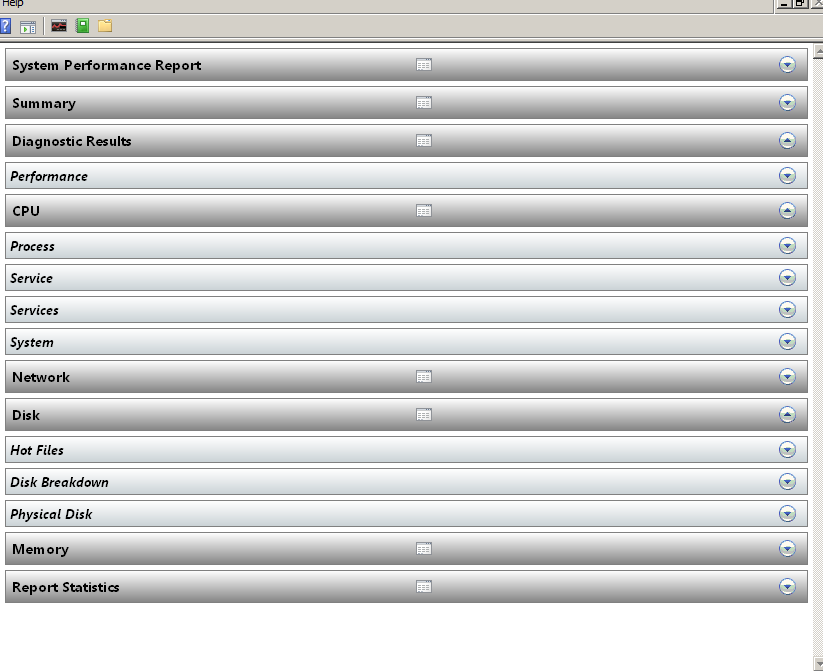
\includegraphics[width=1\textwidth]{c04f03}
	\caption{Menú donde se recogen todos los datos almacenados por categorías.}
	\label{fig:c04f03}
\end{figure}




%----------------------------------------------------------------------------------------
% CUESTION 5
%----------------------------------------------------------------------------------------
\section{Cree un recopilador de datos definido por el usuario (modo	avanzado) que incluya tanto el contador de rendimiento como los datos de 	seguimiento: -Todos los referentes al procesador, al proceso y al servicio web. -Intervalo de muestra 15 segundos. -Almacene el resultado en el directorio Escritorio \\logs. Incluya las capturas de pantalla de cada paso.}

\begin{figure}[H]
	\centering
	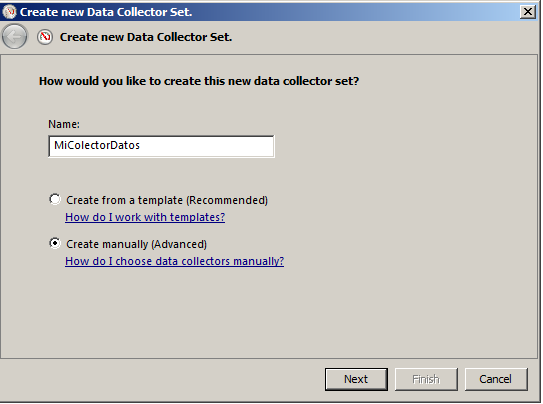
\includegraphics[width=1\textwidth]{c05f01}
	\caption{Iniciando un recopilador personal.}
	\label{fig:c05f01}
\end{figure}
\begin{figure}[H]
	\centering
	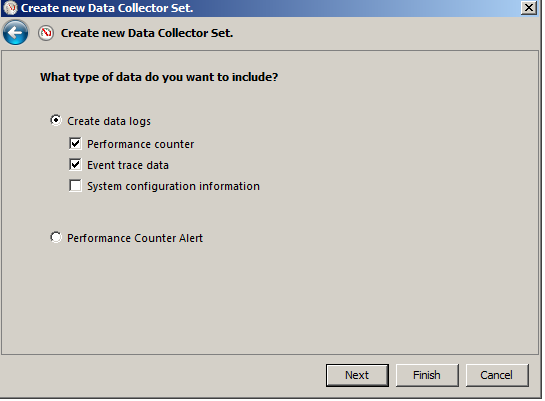
\includegraphics[width=1\textwidth]{c05f02}
	\caption{Tipo de datos que vamos a incluir en el recopilador.}
	\label{fig:c05f02}
\end{figure}
\begin{figure}[H]
	\centering
	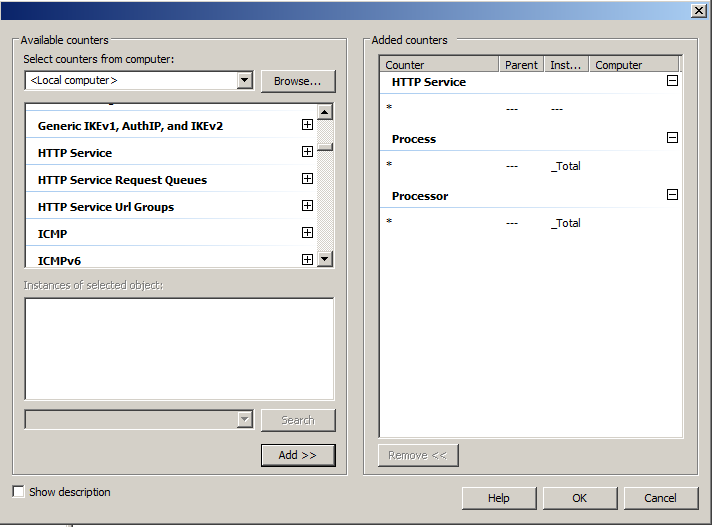
\includegraphics[width=1\textwidth]{c05f03}
	\caption{Datos que vamos a incluir en el recopilador.}
	\label{fig:c05f03}
\end{figure}

\begin{figure}[H]
	\centering
	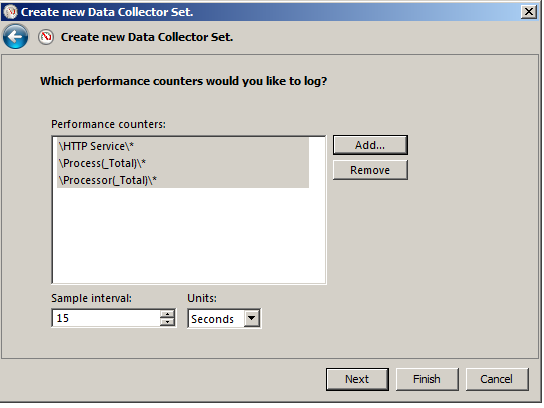
\includegraphics[width=1\textwidth]{c05f04}
	\caption{Intervalo y confirmación de datos a incluir.}
	\label{fig:c05f04}
\end{figure}
\begin{figure}[H]
	\centering
	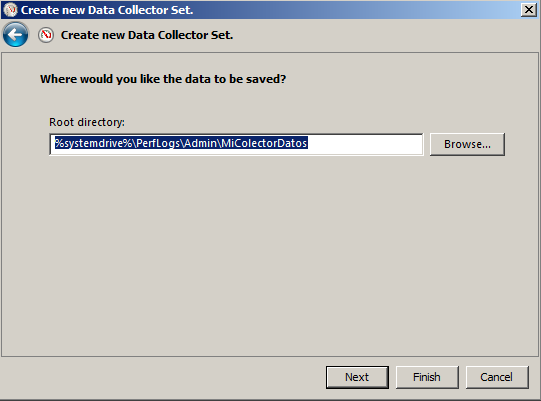
\includegraphics[width=1\textwidth]{c05f05}
	\caption{Fichero de salida de datos.}
	\label{fig:c05f05}
\end{figure}
\begin{figure}[H]
	\centering
	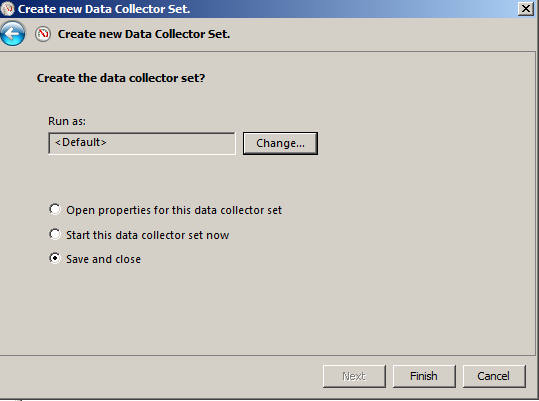
\includegraphics[width=1\textwidth]{c05f06}
	\caption{Finalización de la configuración manual del recopilador de datos.}
	\label{fig:c05f06}
\end{figure}



%----------------------------------------------------------------------------------------
% CUESTION 6
%----------------------------------------------------------------------------------------

\section{Instale alguno de los monitores comentados arriba en su máquina y pruebe a ejecutarlos (tenga en cuenta que si lo hace en la máquina virtual, los resultados pueden no ser realistas). Alternativamente,	busque otros monitores para hardware comerciales o de código abierto para Windows y Linux.}

He elegido para probar el xsensors para linux:

\begin{figure}[H]
	\centering
	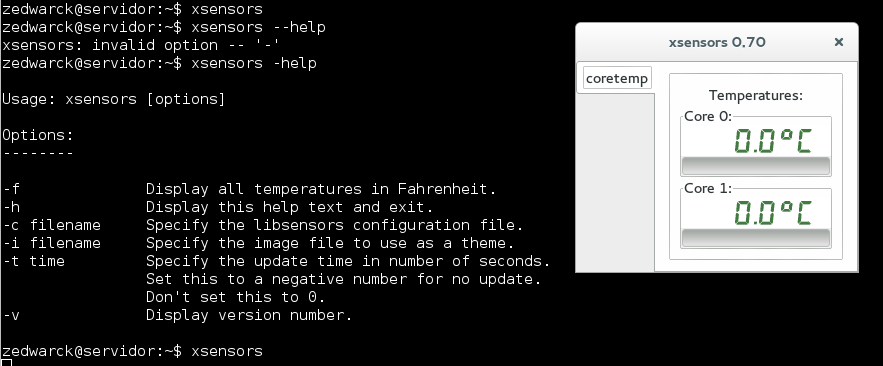
\includegraphics[width=1\textwidth]{c06f01}
	\caption{xsensors ejecutándose junto con los comandos de opciones disponibles.}
	\label{fig:c06f01}
\end{figure}

En la figura podemos ver que no marca temperatura es debido a que estamos corriendo el programa bajo una maquina virtual.

Para linux hay otros incluso bajo consola bastante buenos como es el nmon:
\begin{figure}[H]
	\centering
	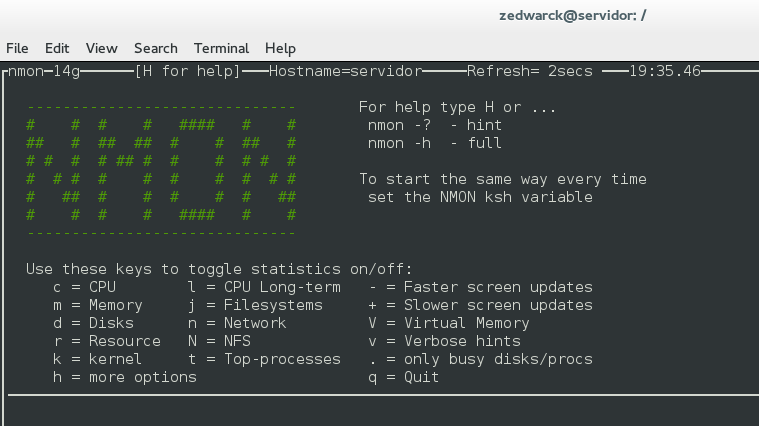
\includegraphics[width=1\textwidth]{c06f02}
	\caption{nmon ejecutándose}
	\label{fig:c06f02}
\end{figure}

Podemos ver como tiene muchos parámetros configurables y poder monitorizar bastantes cosas como por ejemplo la memoria:
\begin{figure}[H]
	\centering
	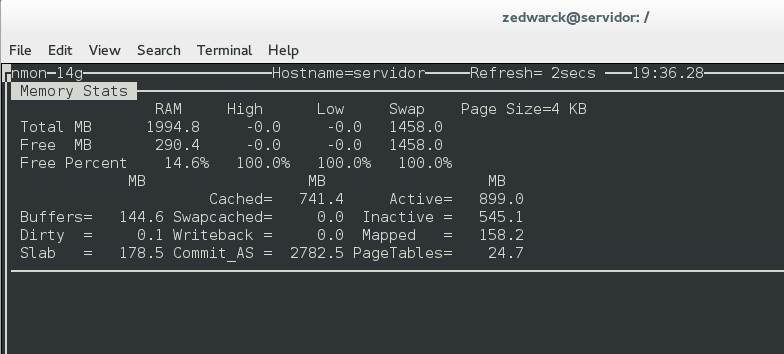
\includegraphics[width=1\textwidth]{c06f03}
	\caption{Monitorización de memoria con nmon.}
	\label{fig:c06f03}
\end{figure}

Para Windows tenemos un amplio repertorio, como por ejemplo:\\
	-Open Hardware Monitor.\\
	-HWMonitor.\\
	

%----------------------------------------------------------------------------------------
% CUESTION 7
%----------------------------------------------------------------------------------------
\section{Visite la web del proyecto y acceda a la demo que proporcionan (http://demo.munin-monitoring.org/) donde se muestra cómo monitorizan un servidor. Monitorice varios parámetros y haga capturas de pantalla de lo que está mostrando comentando qué observa.}	

\begin{figure}[H]
	\centering
	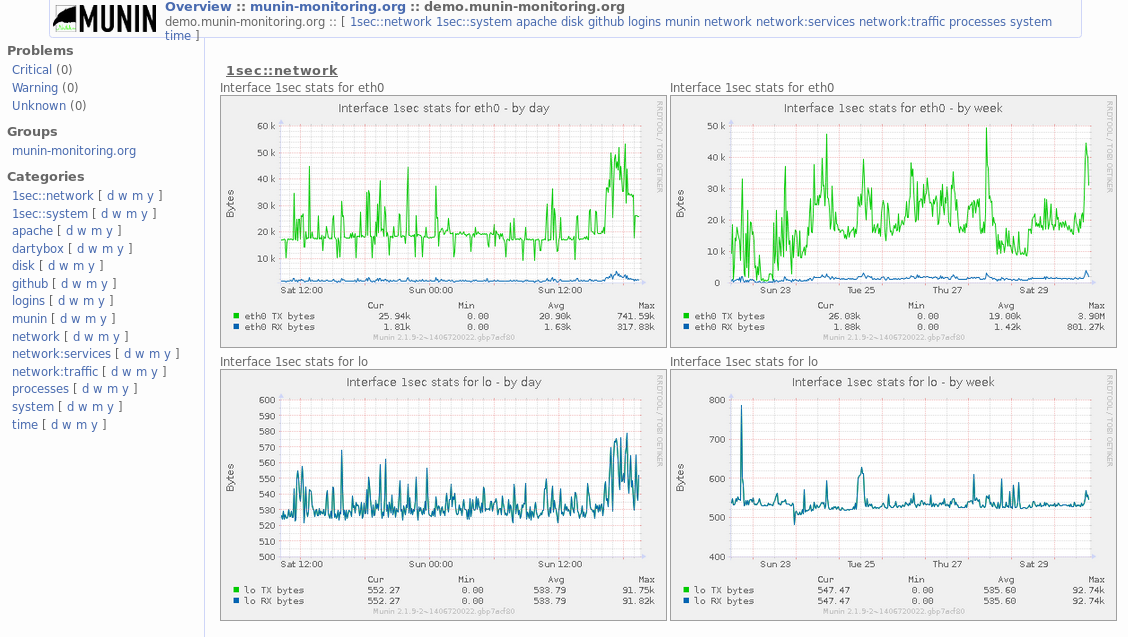
\includegraphics[width=1\textwidth]{c07f01}
	\caption{Monitorización de las interfaces de red desde la webdemo}
	\label{fig:c07f01}
\end{figure}
\begin{figure}[H]
	\centering
	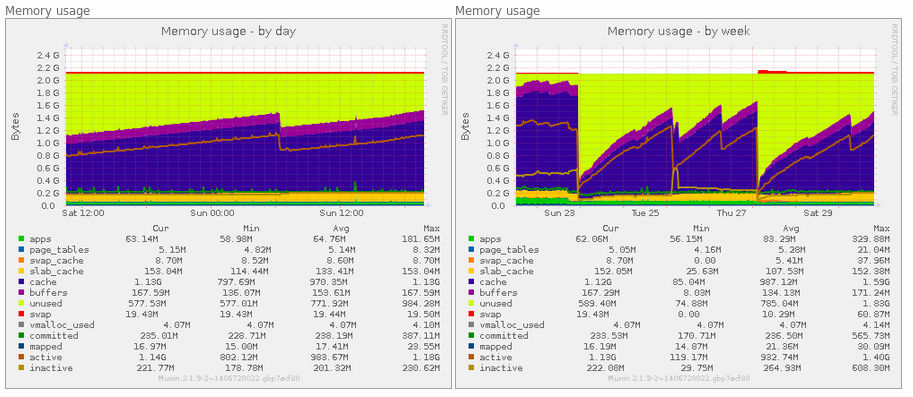
\includegraphics[width=1\textwidth]{c07f02}
	\caption{Monitorización del uso de memoria desde la webdemo}
	\label{fig:c07f02}
\end{figure}

En ambos casos podemos ver 2 gráficas, la primera muestra la monitorización que hemos elegido a lo largo del día y la segunda a lo largo de la semana.\\
En la segunda gráfica de memoria podemos ver caídas de memoria seguramente originadas por reinicios del servidor o caídas del sistema.\\



%----------------------------------------------------------------------------------------
% CUESTION OPCIONAL 2:
%----------------------------------------------------------------------------------------
\section{Instale Nagios en su sistema (el que prefiera)	documentando el proceso y muestre el resultado de la monitorización de su sistema comentando qué aparece. \cite{c02o}}


Para instalar Nagios en Ubuntu primero preinstalamos algunos requisitos. segun el manual habría que poner:\\

sudo apt-get install wget build-essential apache2 php5-gd libgd2-xpm libgd2-xpm-dev libapache2-modphp5\\

Pero vamos a dejar la linea de la siguiente manera para Ubuntu 14.04:\\

sudo apt-get install wget build-essential apache2 php5-gd libgd2-xpm-dev apache2-utils\\

\begin{figure}[H]
	\centering
	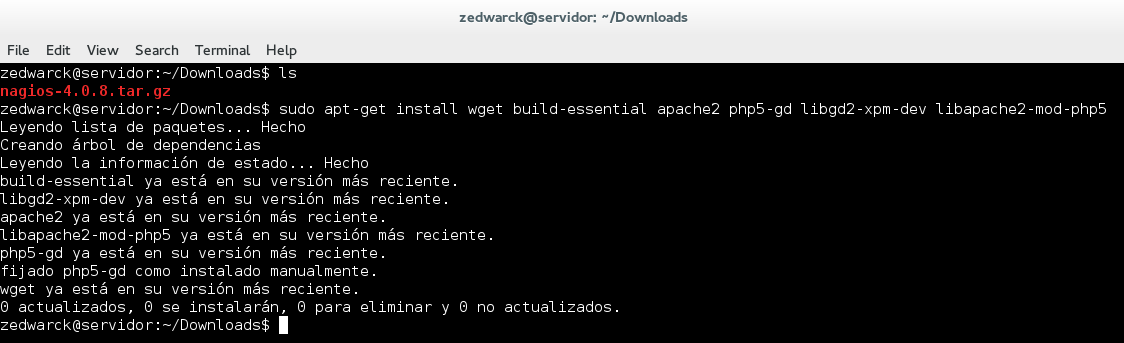
\includegraphics[width=1\textwidth]{co02f01}
	\caption{Prerequisitos de nagios con apt-get.}
	\label{fig:co02f01}
\end{figure}

Luego nos descargamos nagios:\\
cd /tmp\\
wget http://prdownloads.sourceforge.net/sourceforge/nagios/nagios-4.0.4.tar.gz\\
wget http://nagios-plugins.org/download/nagios-plugins-2.0.tar.gz\\

Nos creamos un grupo y un usuario en él que se necesita para su correcto funcionamiento:\\
useradd nagios\\
groupadd nagcmd\\
usermod -a -G nagcmd nagios\\

\begin{figure}[H]
	\centering
	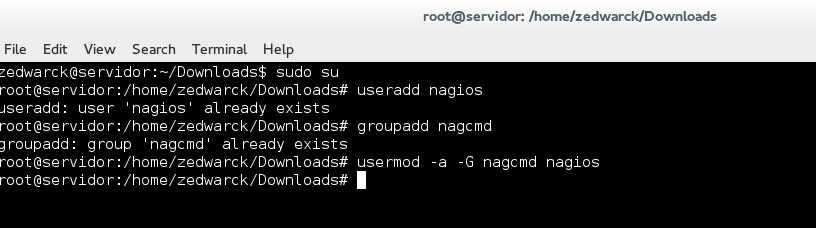
\includegraphics[width=1\textwidth]{co02f02}
	\caption{Creacion de usuario y grupo Nagios.}
	\label{fig:co02f02}
\end{figure}

Descomprimimos:\\
tar zxvf nagios-4.0.4.tar.gz\\
tar zxvf nagios-plugins-2.0.tar.gz\\

\begin{figure}[H]
	\centering
	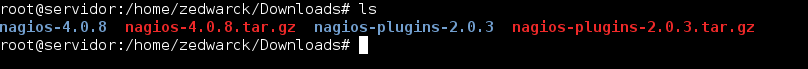
\includegraphics[width=1\textwidth]{co02f03}
	\caption{Archivos de instalación de Nagios descomprimidos.}
	\label{fig:co02f03}
\end{figure}

Accedemos al directorio de instalación y configuramos el instalador:\\

./configure --with-nagios-group=nagios --with-command-group=nagcmd -–with-mail=/usr/bin/sendmail\\

\begin{figure}[H]
	\centering
	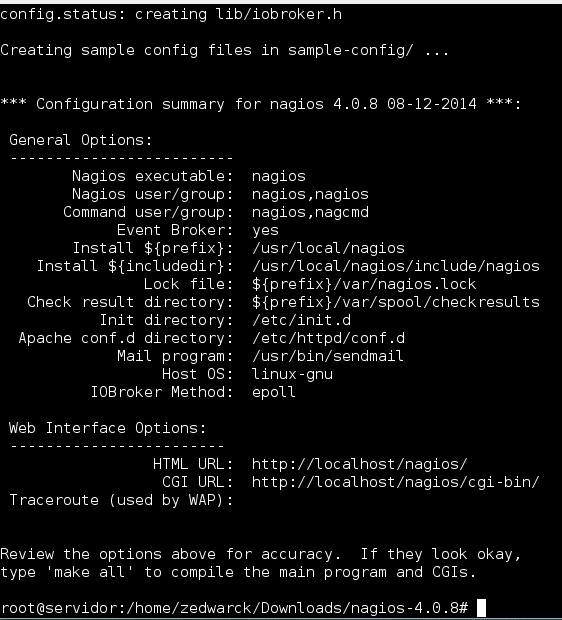
\includegraphics[width=1\textwidth]{co02f04}
	\caption{Preconfiguración de Nagios completada.}
	\label{fig:co02f04}
\end{figure}

Luego hacemos los makes:\\
make all\\
make install\\
make install-init\\
make install-config\\
make install-commandmode\\
make install-webconf\\

\begin{figure}[H]
	\centering
	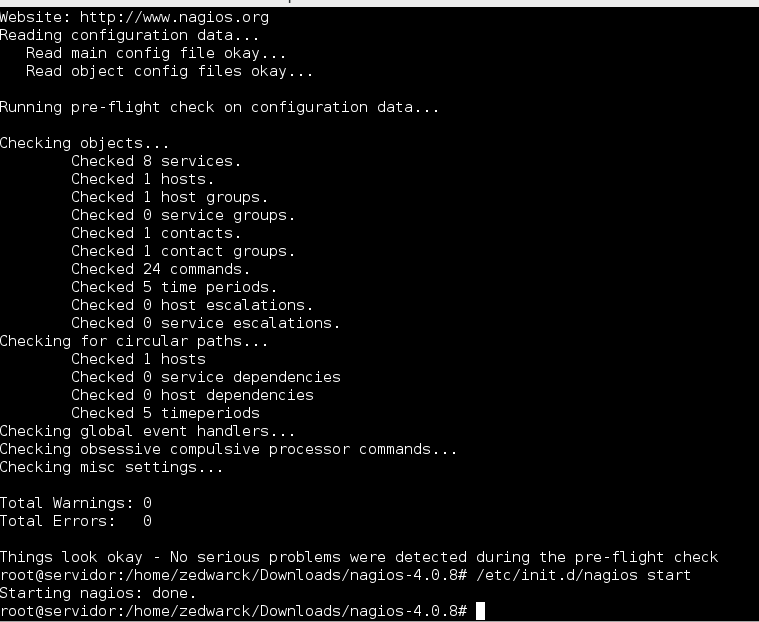
\includegraphics[width=1\textwidth]{co02f05}
	\caption{Instalacion de Nagios completada y servicio corriendo.}
	\label{fig:co02f05}
\end{figure}

El último puede que nos de error, si es así nos creamos el directorio /etc/httpd/conf.d y volvemos a ejecutar el ultimo make. Después de eso nos vamos a ese directorio y copiamos el archivo nagios.conf al directorio de configuraciones de apache: /etc/apache2/conf-enabled/ \\

Finalmente ponemos:\\
cp -R contrib/eventhandlers/ /usr/local/nagios/libexec/ \\
chown -R nagios:nagios /usr/local/nagios/libexec/eventhandlers \\
/usr/local/nagios/bin/nagios -v /usr/local/nagios/etc/nagios.cfg \\

Iniciamos el servicio naglios: service nagios restart \\

Por ultimo reiniciamos apache: service apache2 restart \\


Para poder acceder nos hace falta configurar un usuario:\\

htpasswd –c /usr/local/nagios/etc/htpasswd.users nagiosadmin \\


Y para poder visualizar gráficas nos hace falta el pluging:\\

cd /tmp/nagios-plugins-2.0 \\
./configure --with-nagios-user=nagios --with-nagios-group=nagios \\
make \\
make install \\

Con esto ya casi lo tendríamos todo, solo nos faltaría configurar nuestro apache para que acepte scripts CGI.\\

Para acceder, desde un navegador ponemos la IP o localhost(si esta activo desde el archivo .conf)/nagios:

\begin{figure}[H]
	\centering
	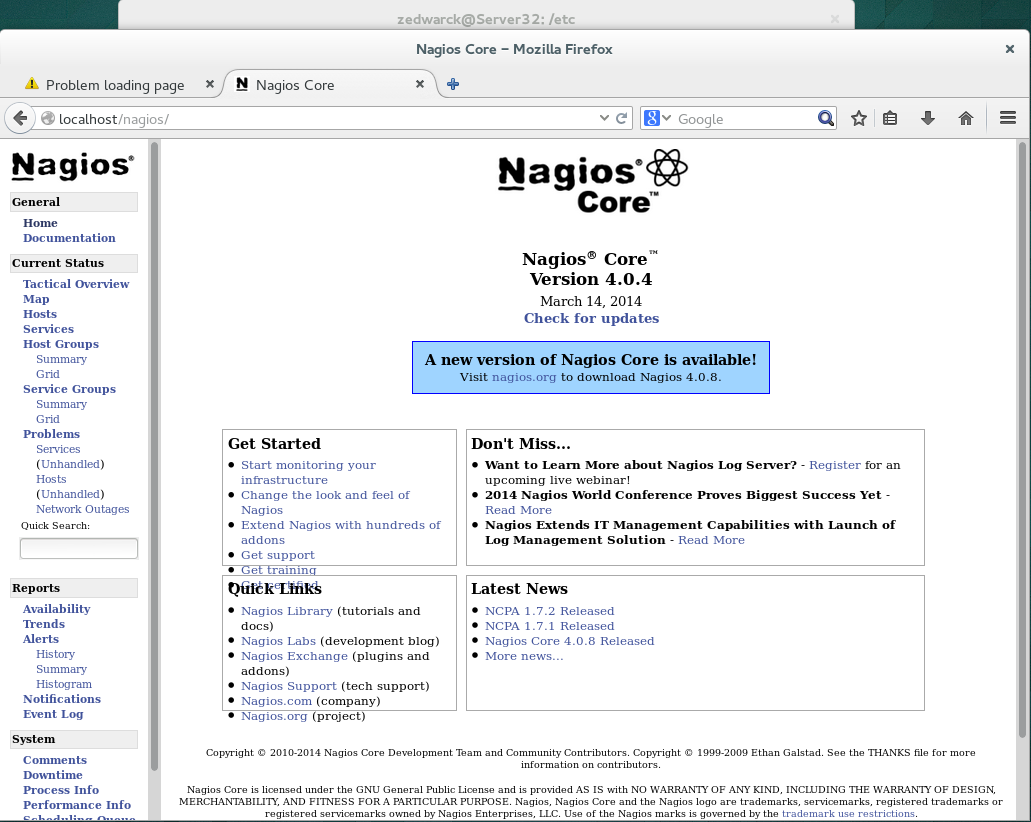
\includegraphics[width=1\textwidth]{nagiosrun1}
	\caption{Home Web de Nagios funcionando.}
	\label{fig:nagiosrun1}
\end{figure}


%----------------------------------------------------------------------------------------
% CUESTION OPCIONAL 3
%----------------------------------------------------------------------------------------
\section{Con Ganglia haga lo mismo que con Munin.}

\begin{figure}[H]
	\centering
	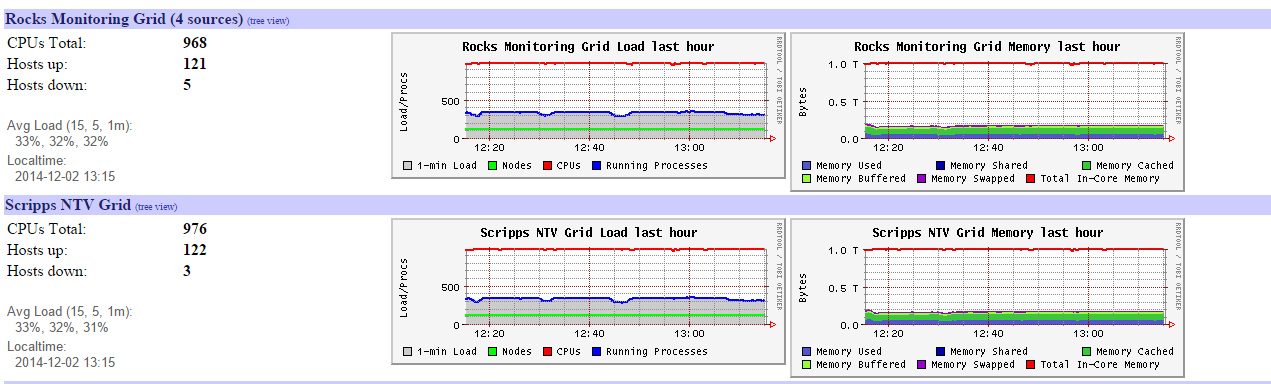
\includegraphics[width=1\textwidth]{co03f01}
	\caption{Monitorización de servidor de pruebas con Munin}
	\label{fig:co03f01}
\end{figure}

%----------------------------------------------------------------------------------------
% CUESTION OPCIONAL 4
%----------------------------------------------------------------------------------------
\section{Prueba a instalar este monitor es alguno de sus tres sistemas. Realice capturas de pantalla del proceso de instalación y comente capturas de pantalla del programa en ejecución.\cite{c04o}}

Instalamos y configuramos nuestro servidor con zabbix siguiendo los pasos indicados en la cita(exceptuando el usuario de la base de datos que en nuestro caso era root).\\
Una vez instalado podemos acceder con el navegador:

\begin{figure}[H]
	\centering
	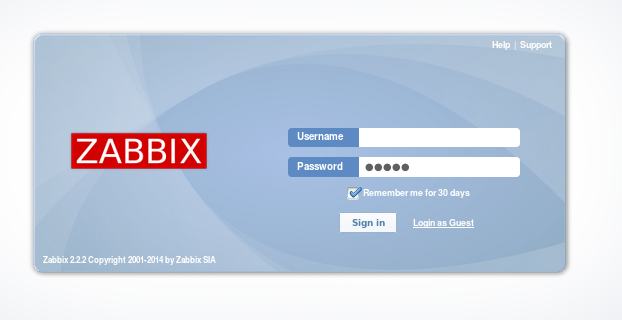
\includegraphics[width=1\textwidth]{co04f01}
	\caption{Pantalla de login de Zabbix.}
	\label{fig:co04f01}
\end{figure}

Introducimos usuario: admin y clave: zabbix, para acceder y ya tendremos la pantalla de inicio:\\
\begin{figure}[H]
	\centering
	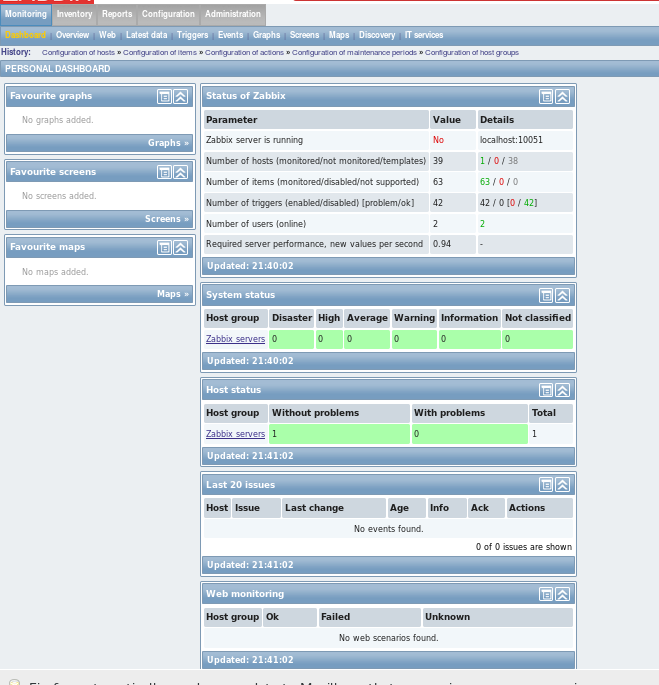
\includegraphics[width=1\textwidth]{co04f02}
	\caption{Pantalla Principal de Zabbix.}
	\label{fig:co04f02}
\end{figure}


%----------------------------------------------------------------------------------------
% CUESTION OPCIONAL 5
%----------------------------------------------------------------------------------------
\section{Pruebe a instalar este monitor en alguno de sus tres sistemas. Realice capturas de pantalla del proceso de instalación y comente las capturas de pantalla 	del programa de ejecución}

Necesitamos tener apache, php5 y mysql como prerequisito, para ello ponemos:\\

sudo apt-get install apache2 php5 mysql-server phpmyadmin\\

Una vez tengamos todo los prerequisitos, instalamos cacti:\\

sudo apt-get install cacti cacti-spine\\

Después de hacer toda la instalación ya ponemos ir a un navegador y poner como dirección: localhost/cacti

\begin{figure}[H]
	\centering
	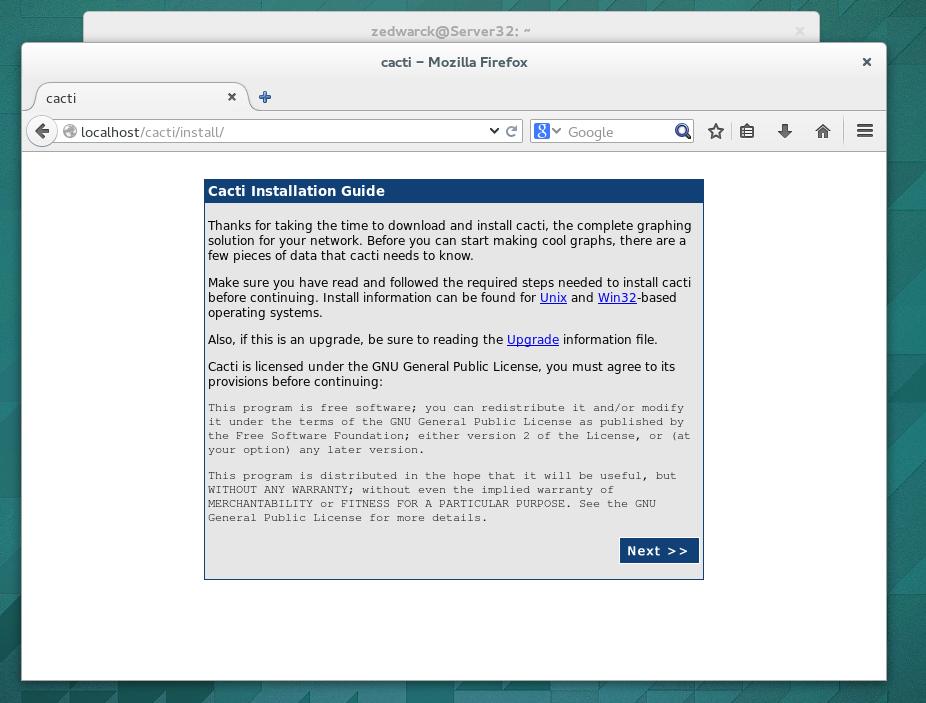
\includegraphics[width=1\textwidth]{co05f01}
	\caption{Pantalla inicial de preinstalación de Cacti.}
	\label{fig:co05f01}
\end{figure}

Pulsamos a siguiente y le decimos que queremos una nueva instalación:

\begin{figure}[H]
	\centering
	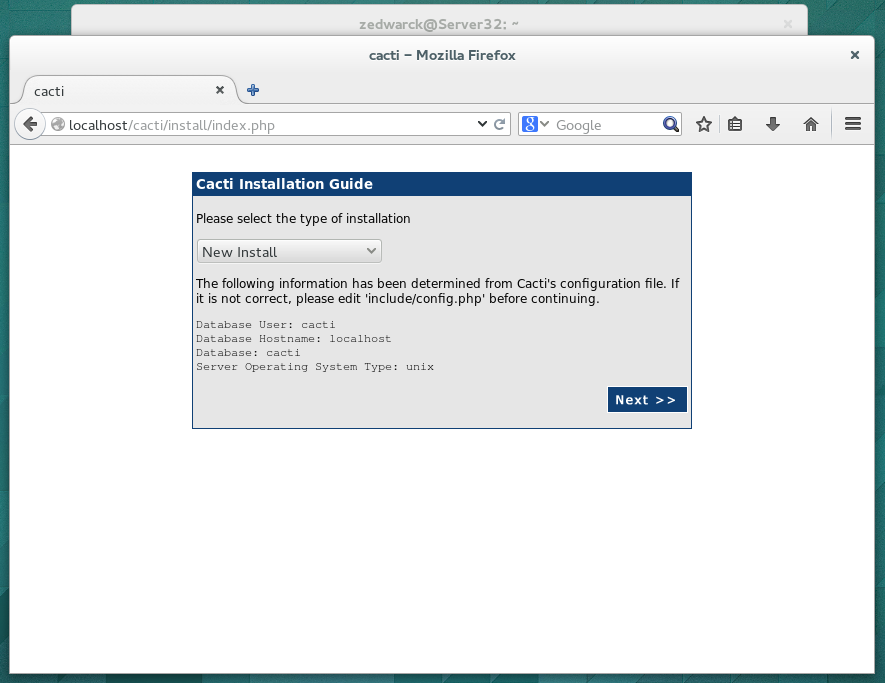
\includegraphics[width=1\textwidth]{co05f02}
	\caption{Opción de nueva instalación o actualización.}
	\label{fig:co05f02}
\end{figure}

Luego el sistema comprueba que están los archivos que necesita en sus rutas adecuadas. Pulsamos terminar para completar el proceso:

\begin{figure}[H]
	\centering
	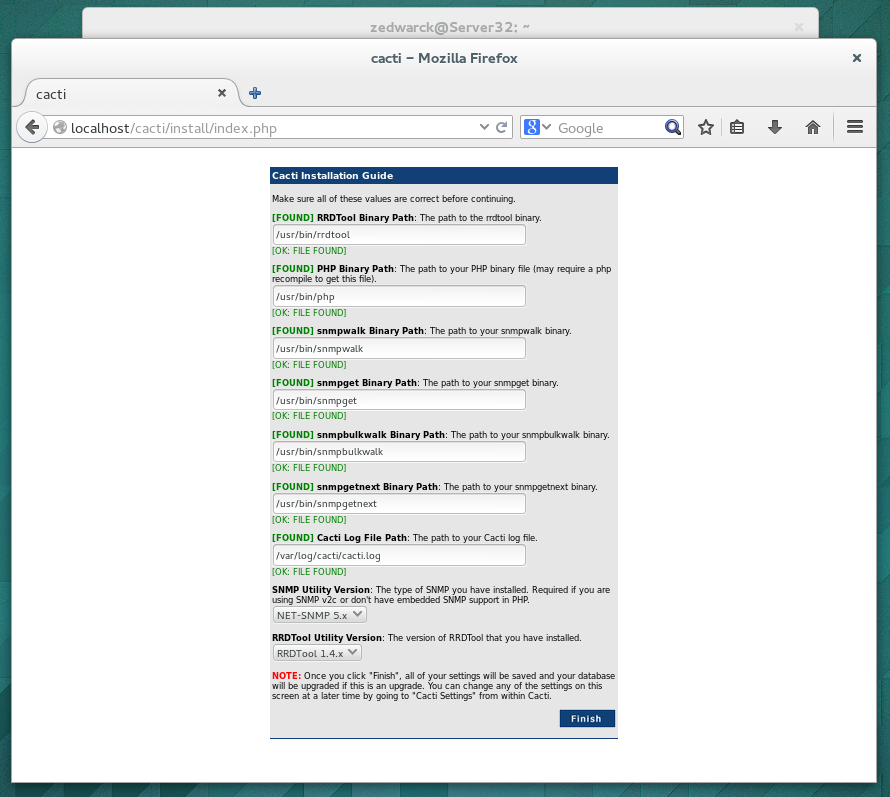
\includegraphics[width=1\textwidth]{co05f03}
	\caption{Comprobación de rutas en la instalación de cacti.}
	\label{fig:co05f03}
\end{figure}

Luego nos pide un usuario y un password que le ponemos "admin admin":

\begin{figure}[H]
	\centering
	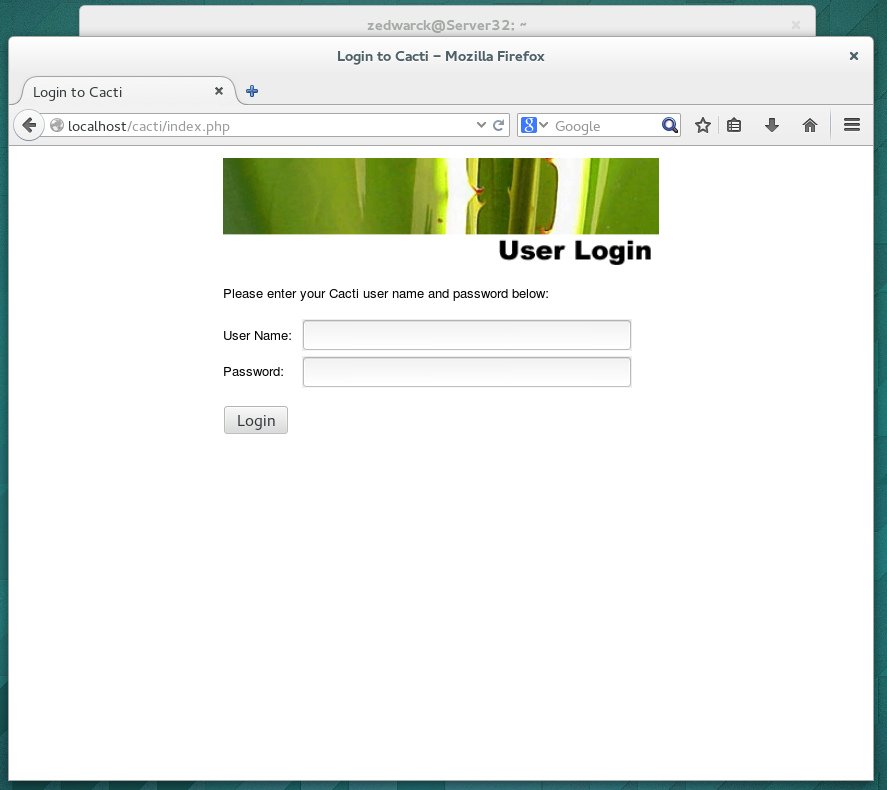
\includegraphics[width=1\textwidth]{co05f04}
	\caption{Login en cacti.}
	\label{fig:co05f04}
\end{figure}

Luego nos obliga a cambiar de password:

\begin{figure}[H]
	\centering
	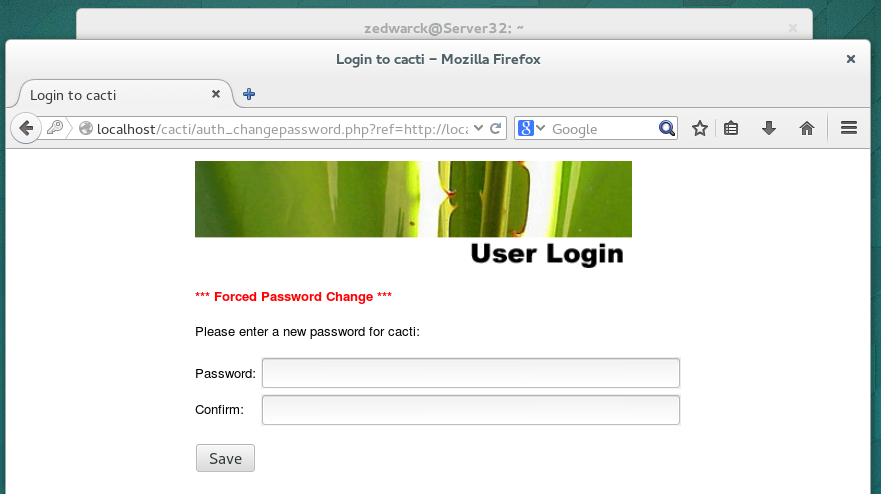
\includegraphics[width=1\textwidth]{co05f05}
	\caption{Cambio de password para admin en cacti.}
	\label{fig:co05f05}
\end{figure}

Finalmente accedemos al entorno web de cacti:
\begin{figure}[H]
	\centering
	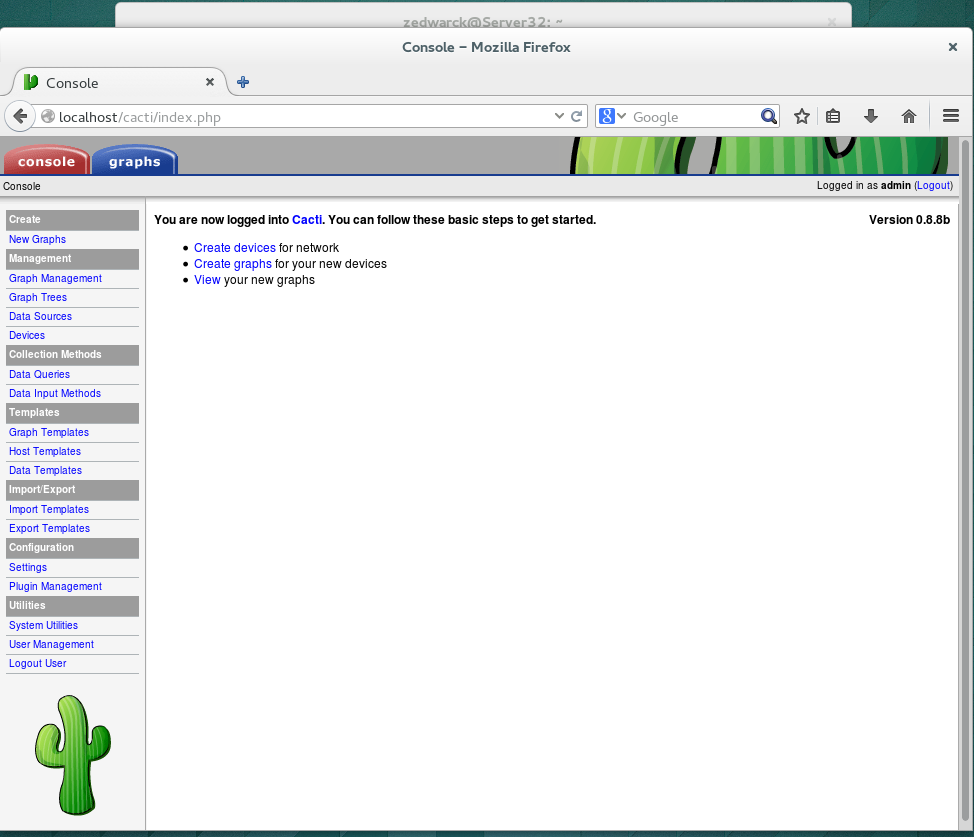
\includegraphics[width=1\textwidth]{co05f06}
	\caption{Home de cacti.}
	\label{fig:co05f06}
\end{figure}

Podemos configurar parámetros de rango de tiempo o que es lo que queremos muestrear en gráficas, en nuestro caso el uso de memoria, la carga media del servidor, usuario logueados y procesos activos:
\begin{figure}[H]
	\centering
	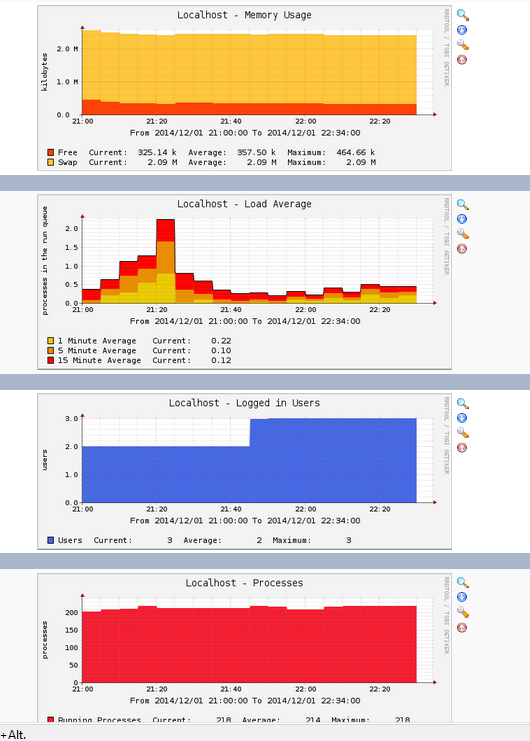
\includegraphics[width=1\textwidth]{co05f07}
	\caption{Gráficas de muestreo en cacti.}
	\label{fig:co05f07}
\end{figure}



%----------------------------------------------------------------------------------------
% CUESTION 8
%----------------------------------------------------------------------------------------
\section{Escriba un breve resumen sobre alguno de los artículos donde se muestra el uso de strace o busque otro y coméntelo}


El comando strace es una utilidad que permite seguir la ejecución de un programa, su eso en principio es sencillo solo poner strace y el nombre del programa a tracear.
En el caso de que la ejecución a estudiar tenga hilos podemos igualmente seguir los hijos del ejecutable mediante el modificador -fF.\\

Una vez visto las trazas de los hijos podemos ver mas concretamente uno de ellos mediante su identificador con el modificador  -p <id>\\

strace acepta como argumentos expresiones generadas con egrep o pgrep para poder seguir por ejemplo a un conjunto de procesos.\\


%----------------------------------------------------------------------------------------
% CUESTION OPCIONAL 7
%----------------------------------------------------------------------------------------
\section{Desarrolle una página en C o C++ y analice su comportamiento usando valgrind. Visite http://www.cs.tut.fi/\~jkorpela/forms/cgic.html para ver un ejemplo sencillo de una página web generada por un programa escrito en C.}

Mi codigo:
\begin{lstlisting}[style=C]
#include <stdio.h>
#include <stdlib.h>
#include <string.h>
#include <time.h>

int main(int argc, char **argv){

	if (argc>6 || argc<5){
		printf("\nERROR. Numero de parametros incorrecto. USO: %s <fila_A> <columna_A> <fila_B> <columna_B> [-v].\n", argv[0]);
		exit(EXIT_FAILURE);
	}

	int f1 = atoi(argv[1]);
	int c1 = atoi(argv[2]);
	int f2 = atoi(argv[3]);
	int c2 = atoi(argv[4]);

	if(c1!=f2){
		printf("\nERROR. Las matrices no son multiplicables. Tamano incorrecto.\n");
		exit(EXIT_FAILURE);
	}

	int i, j, k;
	int suma;
	srand(time(NULL));
	
	//Se crean las matrices y se reserva la memoria
	int **A;
	int **B;
	int **C;
	
	double tiempo;
	struct timespec tiempoI, tiempoF;
	
	A = (int **)malloc(f1*sizeof(int *));
	for(i=0;i<f1;i++)
		A[i]=(int *)malloc(c2*sizeof(int));
	
	B = (int **)malloc(f1*sizeof(int *));
		for(i=0;i<f1;i++)
	B[i]=(int *)malloc(c1*sizeof(int));
	
	C = (int **)malloc(f2*sizeof(int *));
		for(i=0;i<f2;i++)
	C[i]=(int *)malloc(c2*sizeof(int));


	//Se rellenan con enteros aleatorios del 0 al 9
	for (i=0; i<f1; i++)
		for (j=0; j<c1; j++)
		B[i][j] = rand()%10;
	
	for (i=0; i<f2; i++)
		for (j=0; j<c2; j++)
		C[i][j] = rand()%10;
	
	
	//Se multiplica
	clock_gettime(CLOCK_REALTIME, &tiempoI);
	for (i=0; i<f1; i++)
		for (j=0; j<c2; j++){
			suma = 0;
			for (k=0; k<c1; k++)
			suma += B[i][k] * C[k][j];
			A[i][j] = suma;
		}
	clock_gettime(CLOCK_REALTIME, &tiempoF);
	//Se muestra por pantalla la Solucion Completa
	if (argc==6){
		if (strcmp("-v",argv[5])==0){
			for (i=0; i<f1; i++){
				printf("\n");
				for (j=0; j<c2; j++){
					if (A[i][j]>=1000)
						printf("%d",A[i][j]);
					else if (A[i][j]>=100)
						printf(" %d",A[i][j]);
					else if (A[i][j]>=10)
						printf("  %d",A[i][j]);
					else
						printf("   %d",A[i][j]);
				}
			}
		printf("\n");
		}
		else{		
			printf("Parametro opcional incorrecto.\n");
		}
	}
	else{
		tiempo = (double) (tiempoF.tv_sec - tiempoI.tv_sec) + (double) ((tiempoF.tv_nsec - tiempoI.tv_nsec) / (1.e+9));
		
		printf("Tiempo: %8.6f\n",tiempo);
		printf("Componente(0,0): %d\n",A[0][0]);
		printf("Componente(N-1,N-1): %d\n",A[f1-1][c2-1]);
	}

	//Se libera la memoria
	
	for(i=0;i<f1;i++)
		free(A[i]);
	free(A);
	
	for(i=0;i<f1;i++)
		free(B[i]);
	free(B);
	
	for(i=0;i<f2;i++)
		free(C[i]);
	free(C);
	
	return(EXIT_SUCCESS);
	}


\end{lstlisting}


y compilamos con:
\begin{listing}[style=consola, numbers=none]
	$ gcc -o matrices matrices.c
\end{listing}
	
Y finalmente ejecutamos para ver el resultado de valgrind con los parametros adecuados:

\begin{figure}[H]
\centering
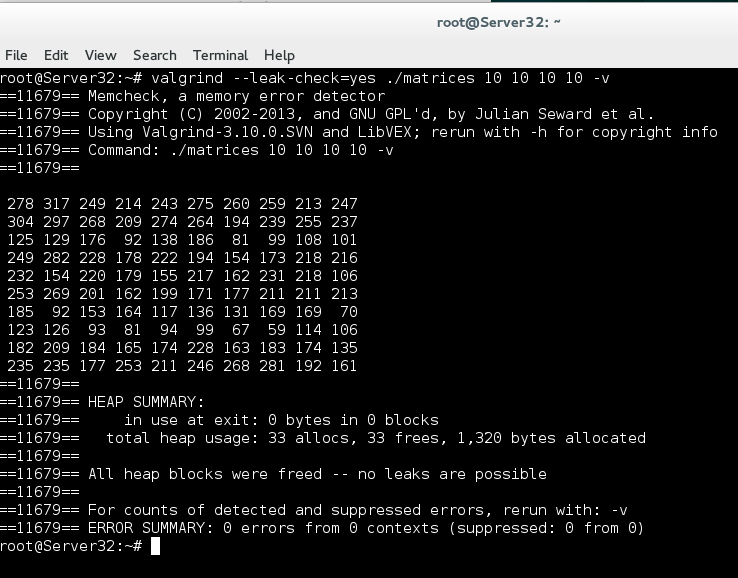
\includegraphics[width=1\textwidth]{co07f01}
\caption{Resultado en consola de valgring sobre un programa de multiplicación de matrices.}
\label{fig:co07f01}
\end{figure}



%----------------------------------------------------------------------------------------
% CUESTION 9
%----------------------------------------------------------------------------------------
\section{Acceda a la consola mysql (o a través de phpMyAdmin) y muestre el resultado de mostrar el ”profile” de una consulta (la creación de	la BD y la consulta la puede hacer líbremente).}

A partir de una base de datos de prueba de poblaciones, países y lenguas en el mundo he creado una consulta la cual esperaba que tardara algo más de lo normal para consultas sencillas. En este caso he sumado la población que habla español en el mundo agrupados por países y he sacado una gráfica. Podemos ver que nos muestra cuanto a tardado, en nuestro caso 0.0032 segundos en realizar toda la consulta.


\begin{figure}[H]
\centering
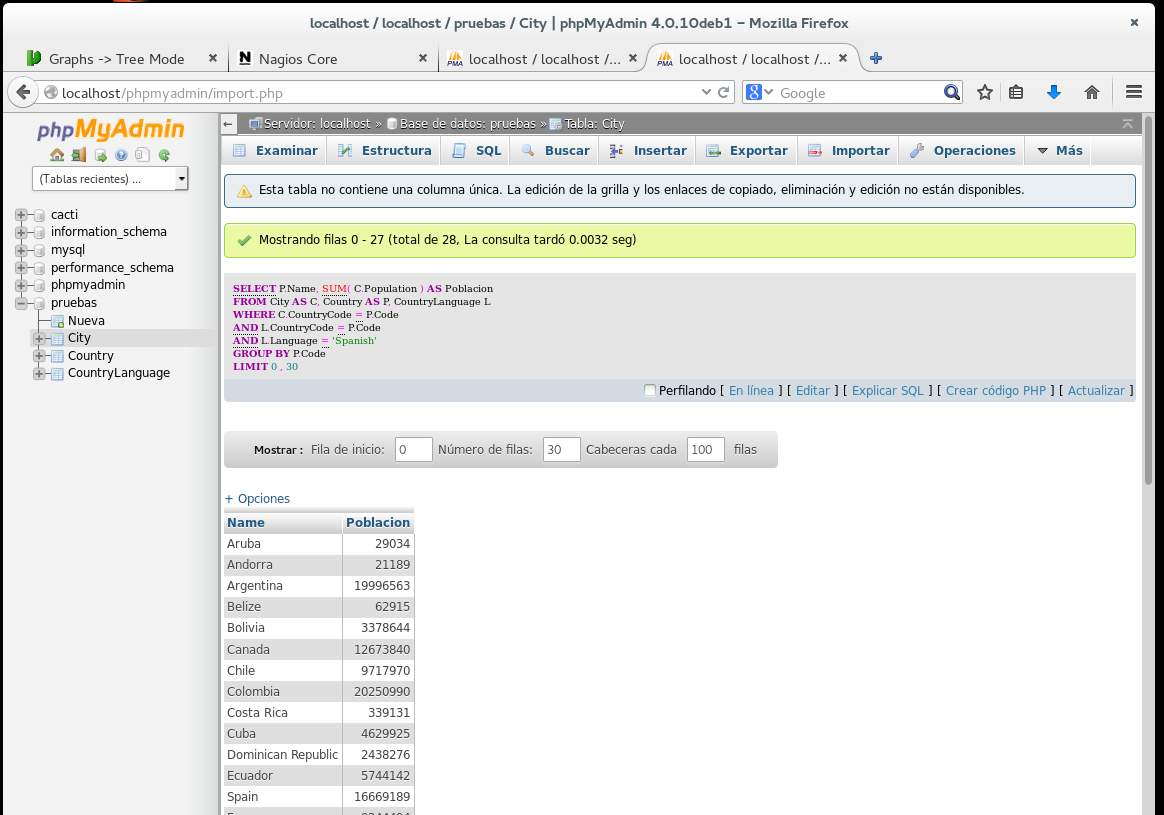
\includegraphics[width=1\textwidth]{c09f01}
\caption{Resultado de la consulta en tabla y el tiempo que a tardado en realizarla.}
\label{fig:c09f01}
\end{figure}

\begin{figure}[H]
\centering
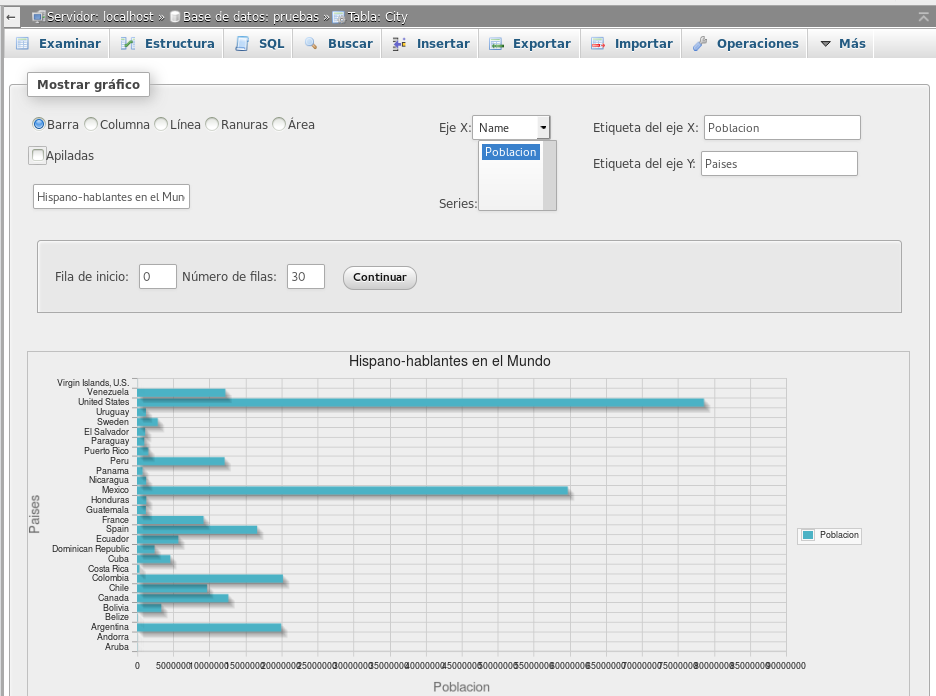
\includegraphics[width=1\textwidth]{c09f02}
\caption{Resultado de la consulta en formato gráfico.}
\label{fig:c09f02}
\end{figure}





%----------------------------------------------------------------------------------------
% CUESTION OPCIONAL 11
%----------------------------------------------------------------------------------------
\section{Al igual que ha realizado el “profiling” con MySQL, realice lo mismo con MongoDB y compare los resultados (use la misma información y la misma consulta, hay traductores de consultas SQL a Mongo). \cite{c11o}}

Instalación de MongoDB:\\

1) Importamos claves: sudo apt-key adv --keyserver hkp://keyserver.ubuntu.com:80 --recv 7F0CEB10\\
2) Importamos repositorios: echo 'deb http://downloads-distro.mongodb.org/repo/ubuntu-upstart dist 10gen' | sudo tee /etc/apt/sources.list.d/mongodb.list \\
3) Actualizamos repositorios: sudo apt-get update\\
4) Instalamos mongoDB: sudo apt-get install -y mongodb-org\\
5) Levantamos servicio: sudo service mongod start\\


Para probar la consulta que creamos para mysql, primero traducimos, he elegido un traductor online \cite{c11o2} y el resultado es de esta consulta MySQL:\\

\begin{listing}[style=consola, numbers=none]
SELECT C.Name, SUM(C.Population) AS Poblacion FROM City As C, Country AS P, CountryLanguage L WHERE C.CountryCode=P.Code AND L.CountryCode=P.Code AND L.Language='Spanish' GROUP BY P.Code
\end{lstlisting}

Se a traducido a:
\begin{listing}[style=consola, numbers=none]

\end{lstlisting}


\clearpage
\bibliography{citas} %archivo citas.bib que contiene las entradas 
\bibliographystyle{unsrt} % hay varias formas de citar


\end{document}